\documentclass[10pt,a4paper,notitlepage]{report}
\usepackage[utf8]{inputenc}
\usepackage{amsmath}
\usepackage{amsfonts}
\usepackage{amssymb}
\usepackage{graphicx}
\usepackage{xcolor}
\usepackage{geometry}
\usepackage{picinpar}
\geometry{a4paper, top=15mm, left=25mm, right=25mm, bottom=25mm, headsep=10mm, footskip=10mm}
%\pagestyle{empty} %keine Kopf-/Fußzeile
\author{Sausage Pan}
\begin{document}
	%Farbdefinierung
	\definecolor{orange}{HTML}{F67800}
	\definecolor{hellorange}{HTML}{FFAD41}
	\definecolor{schwarz}{rgb}{0,0,0}
	%Stildefinitionen!!Wichtig!!
	\newcommand{\Eins}[1]{\color{orange}\textbf{{\Large#1}}} %Überschrift 1. Ordnung
	\newcommand{\Zwei}[1]{\color{orange}\textbf{{\large#1}}} %Überschrift 2. Ordnung
	\newcommand{\Drei}[1]{\color{orange}{\normalsize#1}} %Überschrift 3. Ordnung
	\newcommand{\Text}{\color{schwarz}} %normaler Fließtext
	\newcommand{\Fusszeile}
	{\textit{{\footnotesize Eckert, Georg - Roscher, Philipp - Krien, Alexandra - Sinakow, Sergej - Blasberg, Bettina - Groß, Stephanie Sara}}} %Fußzeile immer am Ende der Seite einfügen!
	%Randstreifen
	\marginpar{\vspace{3.0mm} \color{orange}\rule{0.8mm}{53.3mm} \\[3mm] \color{hellorange}\rule{0.8mm}{170mm}}
	%Header-Bild
	\begin{center}
		
\includegraphics[width=160mm]{header2}
	\end{center}
	%Eigentlicher Inhalt :D

	\Eins{Storyboard}\\
	\\
	\Zwei{Titel:} \Text{Prisma}\\
	\\
	\Zwei{Thema:} \Text{Farbenlehre}\\
	\\
	\Zwei{Zielgruppe:} \Text{Schüler der fünften Klasse}\\
	\\
	\Zwei{1. Grundlegender Aufbau des Spiels}\\
	\\
	\Drei{1.1 Setting}\\
	\Text
	\begin{window}[0,r, 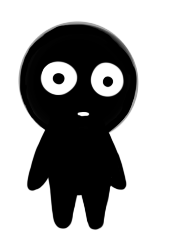
\includegraphics[width = 0.2\textwidth]{maincharacter.png}, ]
	%\parpic[r]{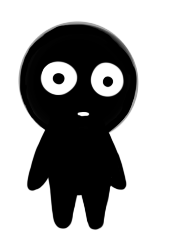
\includegraphics[width = 0.2\textwidth]{maincharacter.png}}
		Das Spiel bewegt sich in einer fiktiven Welt. Der Spieler übernimmt dabei die Rolle eines namenlosen Helden, 
	welcher weder hinsichtlich des Alters, Geschlechts etc. spezifiziert wird.\\\\
	Ausgangssituation für das Spiel ist, dass in Folge eines Missgeschickes der Regenbogen in Fragmente zerspringt.
	Als Resultat wird die Welt in ein einheitliches Grau getaucht.\\\\
	Aufgabe ist es nun, diese Fragmente wieder einzusammeln um letztendlich den Regenbogen neu zusammensetzen zu können. 
	Diese Fragmente finden sich in den einzelnen Level wieder, die als Jump'n'Run angelegt werden.\\\\
	Der Spieler soll dabei ein grundlegendes Verständnis für die Farbenlehre erhalten.\\ 
	Jedes Level fokussiert sich dabei auf ein anderes Teilthema.\\\\
	Als unterstützende Hilfe steht dem Spieler stets eine Art Mentor zur Verfügung, welcher um Hilfe gebeten werden kann. 
	So wollen wir möglicherweise aufkommenden Frust eindämpfen.\\\\
	Gerne würden wir einige Zwischenlevel einbauen, die andere Spielmechaniken nutzen. 
	Denkbar wären hier kleinere Puzzle oder Quiz, um das Wissen zu festigen. \\\\
	Dies haben wir bisher allerdings als optionalen Inhalt deklariert und wollen uns zunächst um die Hauptlevel kümmern. 
	Je nach verbleibender Zeit werden danach die Zwischenlevel konzipiert.\\
	Der Spielfortschritt wird als Farbkreis angezeigt. Dieser ist am Anfang komplett grau. Nachdem eine Farbe in einem Level gewonnen wurde,
	erscheint diese schließlich auch im Farbkreis.
	\end{window}
	\clearpage\
	\marginpar{\vspace{3.0mm} \color{orange}\rule{0.8mm}{53.3mm} \\[3mm] \color{hellorange}\rule{0.8mm}{170mm}}
	\\
	\Drei{1.2. Spielmechaniken}\\
	\\
	\Text
		Das Spiel wird mit 9 Grundmechaniken auskommen. Die ersten zwei sind genretypisch laufen und springen. 
	Dazu kommt das Verschieben von Gegenständen. Die Farblehre wird durch die Prinzipien der additiven und subtraktiven Farbmischung, 
	sowie der Brechung von Licht vermittelt.\\
	\\
	Das erfordert folgende Spielmechanik:\\
	\begin{itemize}
	\item Einfärben des zu Beginn schwarzen Charakters bei Kontakt mit einer Lichtfarbe in dieselbe
	\item additive Farbmischung bei aufeinanderfolgendem Kontakt mit verschiedenen Lichtfarben
	\item Einfärben des Charakters bei Kontakt mit farblichen Flüssigkeiten in dieselbe
	\item subtraktive Farbmischung bei Kontakt mit verschiedenen Flüssigkeiten
	\item Entfernung von Farbpigmenten bei Kontakt mit farbloser Flüssigkeiten
	\item Aufspaltung von Lichtstrahlen in ihr Farbspektrum durch Prismen
	\item Besiegen von Gegnern durch Sprünge bei vorherigem Einfärben mit der Komplementärfarbe
	\item Verdeckung durch Gegenstände, welche vor Lichtstrahlen geschoben werden
	\end{itemize}\
	\\
	\Drei{1.3. Steuerung}\\
	\\
	\Text
		Gespielt wird mit Maus und Tastatur.\\
	Innerhalb der Level kann sich der Spieler über die Pfeiltasten bewegen.
	\clearpage\
	\marginpar{\vspace{3.0mm} \color{orange}\rule{0.8mm}{53.3mm} \\[3mm] \color{hellorange}\rule{0.8mm}{170mm}}
	\\
	\Zwei{2. Ablauf}\
	\\
	\\
	\Text
	\underline{Animation 1 - Introsequenz}\
	\\
	\\
		Grundlegende Story:\\
	\begin{flushright}
	\textit{Eine kleine Motte träumt davon einst so schön wie die strahlend bunten Schmetterlinge zu sein. Gedankenversunken bemerkt sie 
	die Ähnlichkeit zwischen den Schmetterlingen und den bunten Farben des Regenbogens. Überzeugt dass dieser auch ihr prächtige Flügel verleihen könnte, 
	fliegt sie zu ihm hinauf. Durch ein Versehen jedoch zerfällt der Regenbogen in Einzelteile und stürzt zu Boden. \\
	Die Welt wird in ein tristes Grau getaucht. Bewusstlos stürzt die Motte gemeinsam mit einem Regenbogenfragment vor die Füße unseres Protagonisten.}
	\end{flushright}\
	\\
	\underline{Level 1}\\\\\
	\textbf{Thema:}\
	Subtraktive Farbmischung
	\\\\
	\textbf{Farbe:} Blau\
	\\\\
	\textbf{Aufgabe:}\
		Der Protagonist findet sich auf einer Wiese wieder. Die Welt um ihn erscheint in verschiedenen Grautönen. In der Ferne erhebt sich auf einem Hügel ein 		mächtiges, blaues Tor. Der Spieler bewegt die Figur so durch das Level, dass sie sich durch verschiedenfarbige Flüssigkeiten entsprechend einfärbt. Nur wenn 		er zuletzt die Farbe Blau besitzt öffnet sich das Tor und gibt den Weg in das nächste Level frei. Der Spieler überwindet verschiedene Hindernisse. Durch 			Einfärben mit allen Farben färbt er die Figur letztendlich schwarz und begreift so das Prinzip der additiven Farbmischung. Erst wenn das geschehen ist, lässt sich 	die Figur abermals blau färben und das Level abschließen.
	\\\\
	\underline{Animation 2}\
	\\
	\begin{flushright}
	\textit{Die Motte schließt sich dem Protagonisten an und weist ihn zum nächsten Teil, da sie selbst ihr Missgeschick nicht beseitigen kann.\\
	Einführung der Motte als Symbol am unteren Bildschirmrand. Über dieses können von nun an kurze Hilfestellungen abgerufen werden.\\
	Hauptbildschirm als Navigationsfläche. Hier können nun das nächste Level angewählt, eventuelle Achievements angesehen und einige 
	Informationen abgerufen werden.}
	\end{flushright}\
	\\\\
	\underline{Level 2}\\\\\
	\textbf{Thema:}\
	Additive Farbmischung
	%\parpic[r]{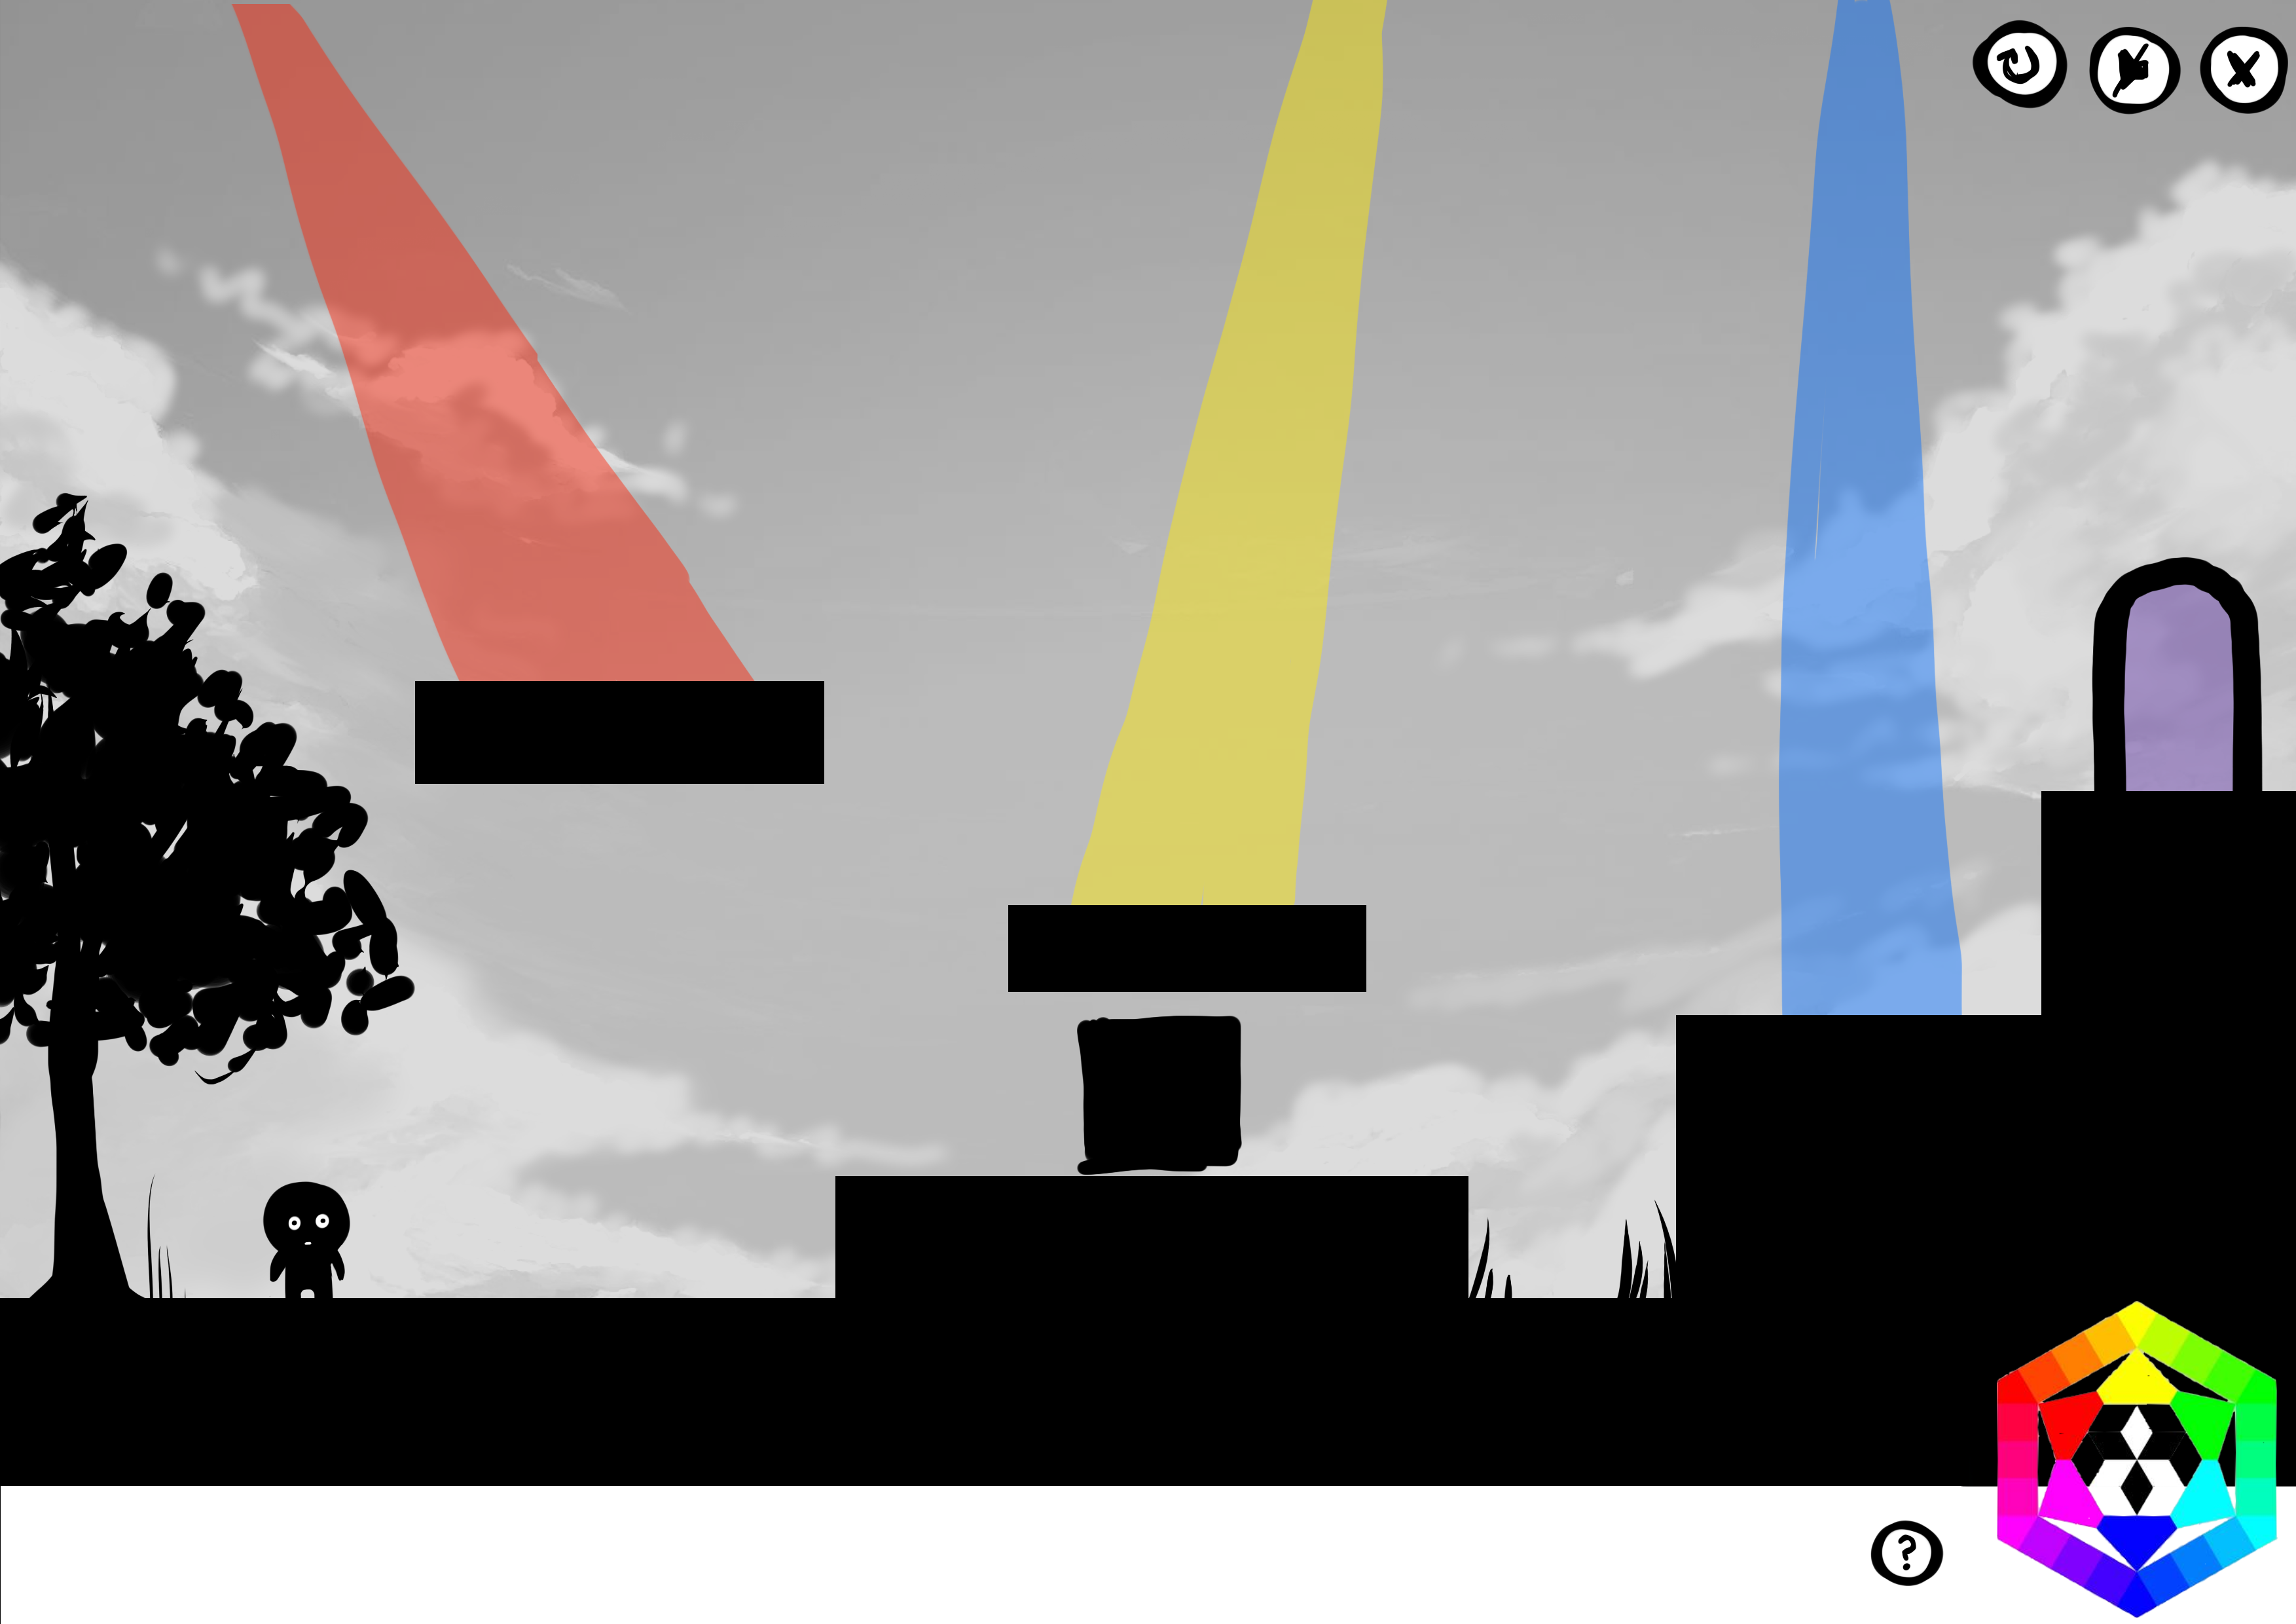
\includegraphics[width = 0.4\textwidth]{level2.png}}\
	\\ 
	\textbf{Farbe:} Rot\
	\\\\
	\textbf{Aufgabe:}\	
	\begin{window}[0,r, 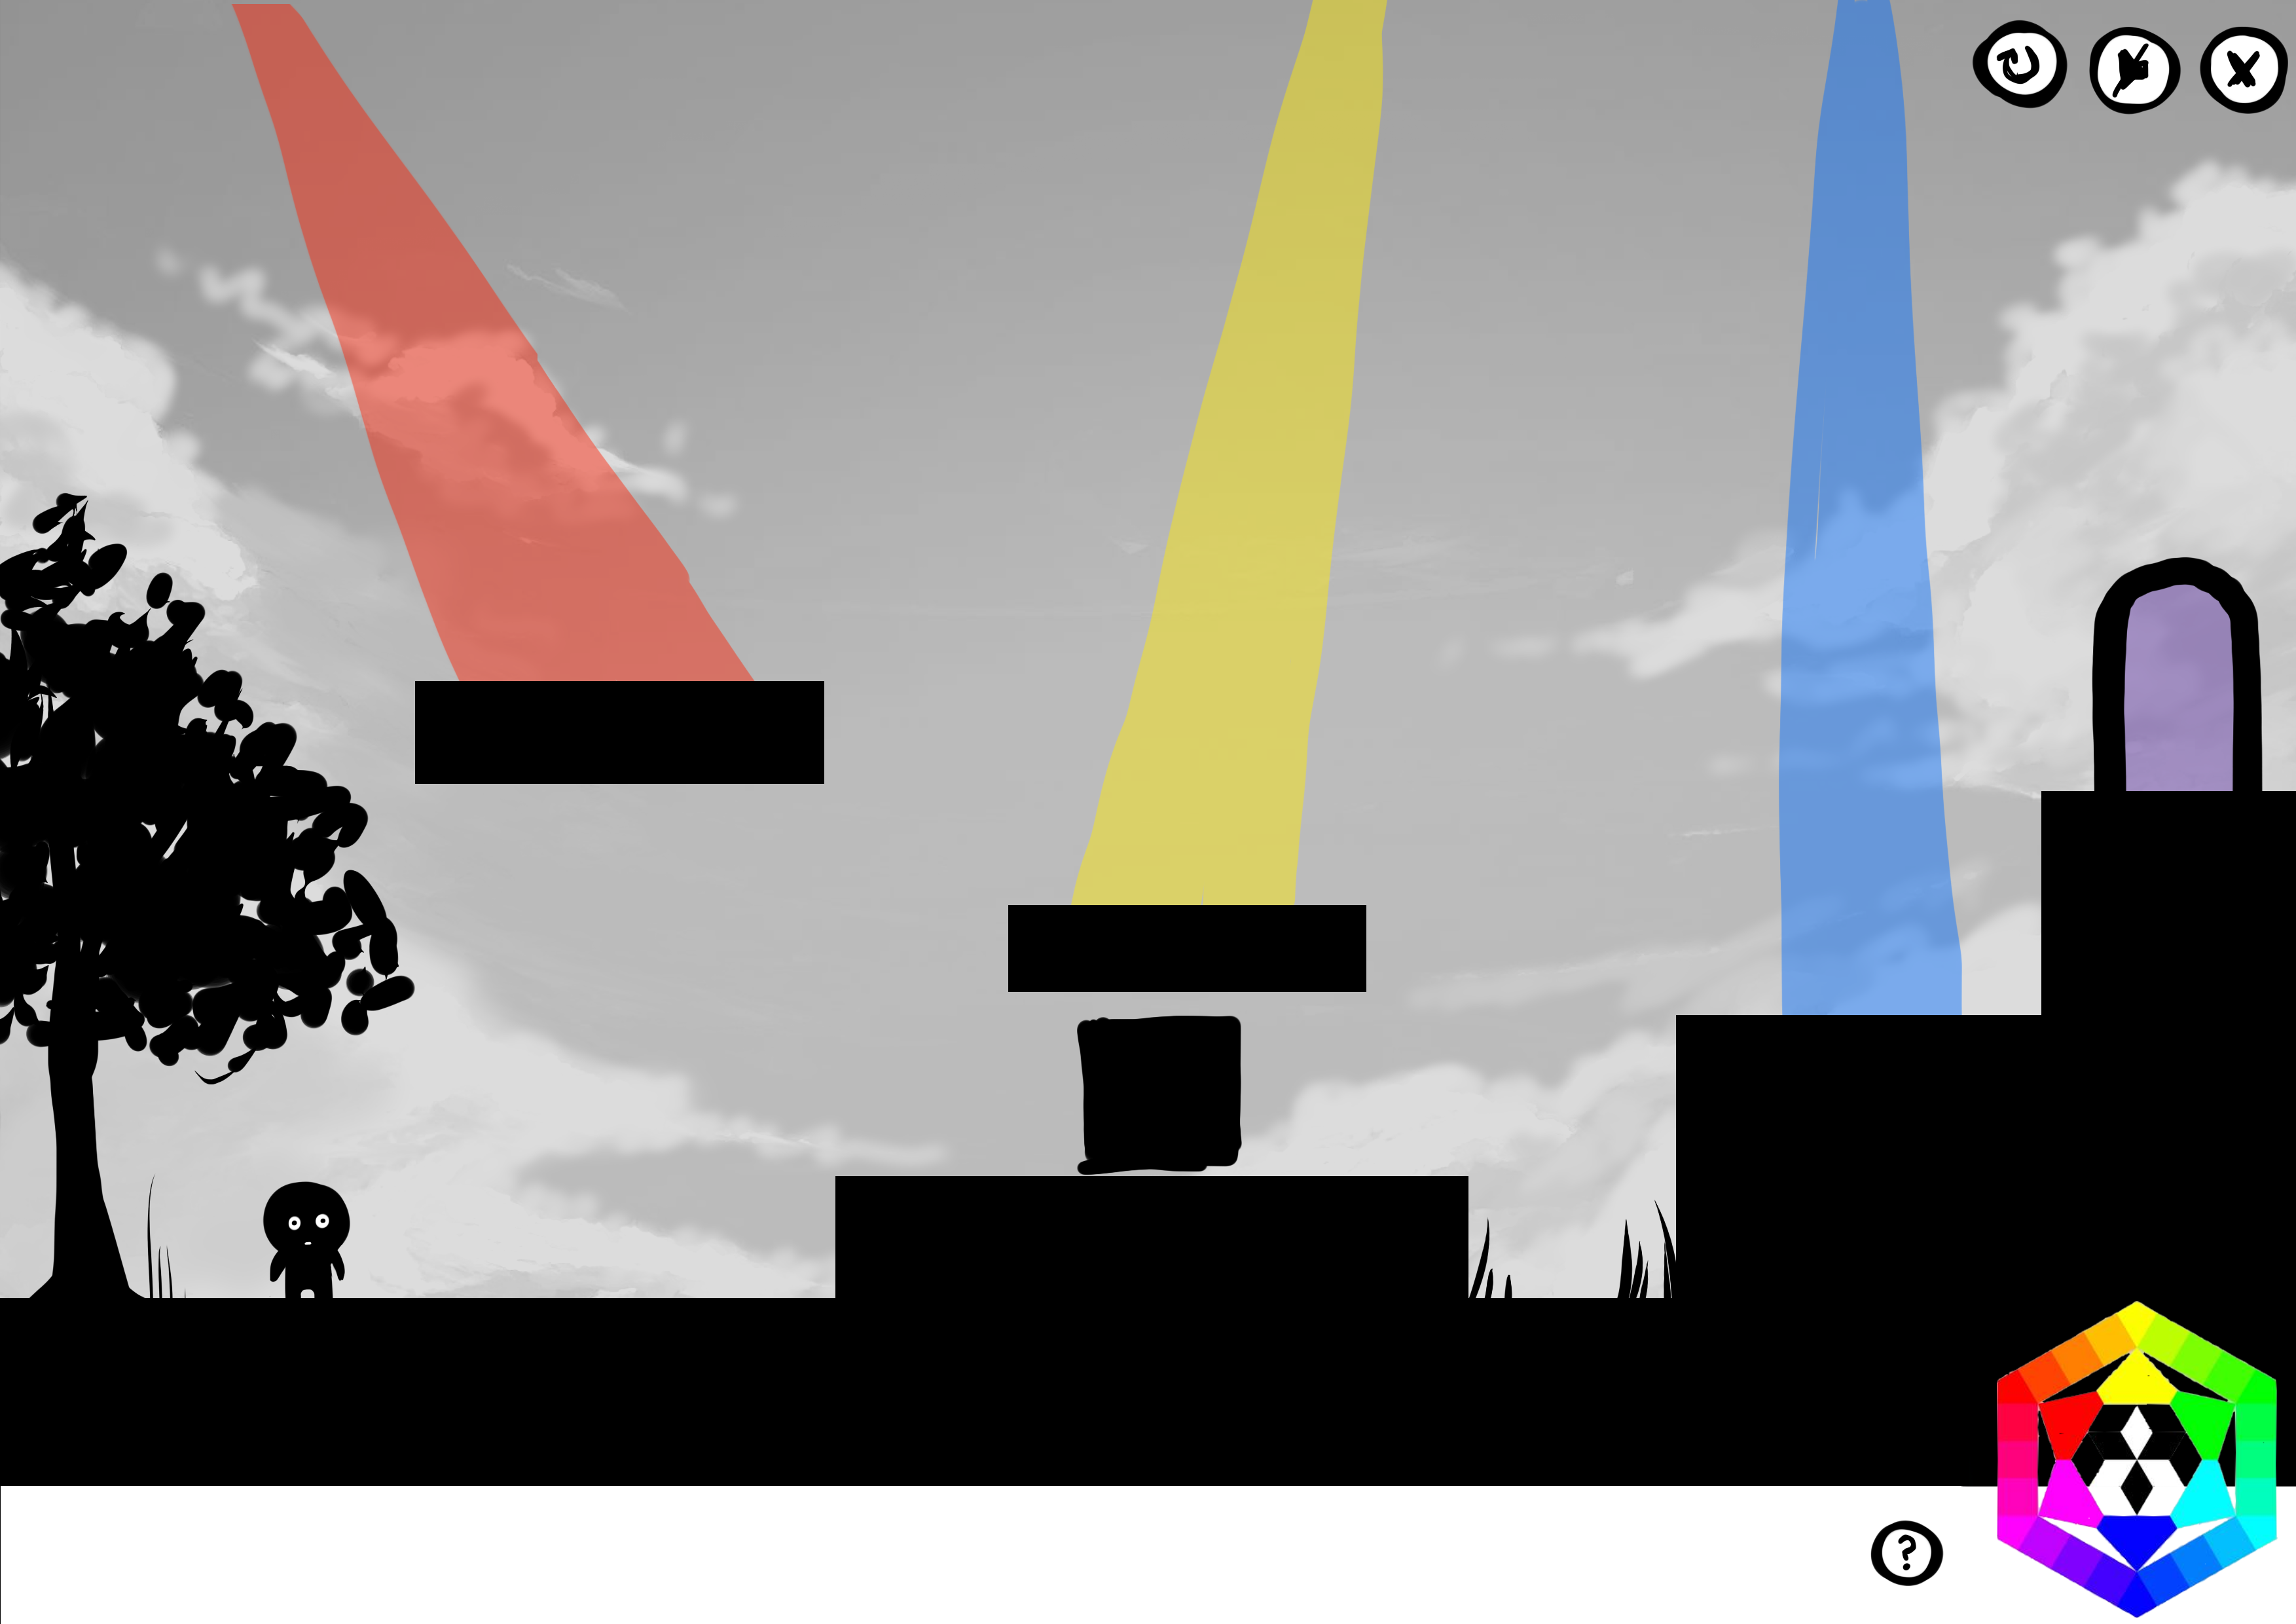
\includegraphics[width = 0.4\textwidth]{level2.png}, ]
	Der Protagonist befindet sich wieder in einem optisch ähnlichen Jump'n'Run Level.\\
	Verschiedene Lichtkegel, die in Grundfarben leuchten, befinden sich in Sichtweite - ebenso ein Tor in einer Mischfarbe.
	Der Spieler muss nun die Figur so durch das Level lotsen, dass sich die Figur in der gleichen Farbe wie das Tor einfärbt. 
	Dazu muss er das Prinzip der additiven Farbmischung anwenden und die Figur so durch die unterschiedlichen Lichtkegel führen, dass die Mischfarbe der betretenen Lichtfarben, die Gesuchte ergibt.\\
	\end{window}
	
	\clearpage\
	\marginpar{\vspace{3.0mm} \color{orange}\rule{0.8mm}{53.3mm} \\[3mm] \color{hellorange}\rule{0.8mm}{170mm}}
	\\
	\underline{Level 3}\\\\\
	\textbf{Thema:}\
	Absorption
	\\\\
	\textbf{Farbe:} Gelb\
	\\\\
	\textbf{Aufgabe:}\
	Der Spieler lernt anhand von farbigen Wolken wie Licht/Farb-Absorbierung funktioniert.
	Es wird erst mittels einer einzigen Wolkenschicht demonstriert wie sich diese auf das einfallende farblose oder farbige Licht auswirkt.\\
	Danach muss der Spieler mehrere Schichten von Wolken so sortieren, dass eine bestimmte Farbe übrig bleibt und er sich gelb färben kann.\\
	Die Wolken werden mithilfe von Schaltern gesteuert.\\
	\\
	\underline{Level 4}\\\\\
	\textbf{Thema:}\
	Komplementärfarben
	\\\\
	\textbf{Farbe:} Grün\
	\\\\
	\textbf{Aufgabe:}\
	Ab diesem Level lernt der Spieler Komplementärfarben kennen. Dies bedeutet, dass der Hauptcharakter immer wieder auf Gegner trifft, die ihm den Weg blockieren. Um diese besiegen zu können muss der Spieler sich mit der Komplementärfarbe seines Gegners einfärben (Feinde sind resistent gegen alle Farben, außer ihrer Komplementärfarbe). 
	\\\\
	\underline{Level 5}\\\\\
	\textbf{Thema:}\
	Warme/Kalte Farben
	\\\\
	\textbf{Farbe:} Cyan\
	\\\\
	\textbf{Aufgabe:}\
	Der Spieler wendet bisher erworbene Kenntnisse an und muss zusätzlich warme und kalte Farben (vor allem Rot und Blau) einsetzen um Hindernisse zu 			überwinden. So sollen eventuell Eisblöcke mit rot geschmolzen, Feuer mit blau durchquert und rot auf Eisbrücken vermieden werden.
	\\\\
	\underline{Level 6}\\\\\
	\textbf{Thema:}\
	Lichtbrechung
	\\\\
	\textbf{Farbe:} Magenta\
	%\parpic[r]{\includegraphics[width = 0.4\textwidth]{lichtbrechung.png}}\
	\\
	\textbf{Aufgabe:}\
	\begin{window}[0,r, \includegraphics[width = 0.4\textwidth]{lichtbrechung.png}, ]
	Der Protagonist befindet sich in einem Raum, wo es nur weiße Lichtkegel gibt. Nebenbei gibt es auch ein paar Prismen, die der Protagonist zu den Lichtkegeln 		schieben muss. Die Idee dabei ist, zu zeigen, wie das Licht anhand des Prismas bricht.\\
	Weiß wird in verschiedene Farben geteilt, da deren Strahlen verschiedene Brechungen haben. Der Spieler muss intuitiv verstehen, dass jede Farbe in 			verschiedenen Winkeln reflektiert wird, nachdem es durch das Prisma gelangt.\\
	Um das Spiel mit den Winkeln zu verstärken, werden Spiegel hinzugefügt. So kann der Spieler bestimmte Lichtstrahlen zu bestimmten Punkten lenken, 
	nachdem das Prisma das weiße Licht in verschiedene Farben geteilt hat.
	\\\\
	\end{window}
	\clearpage\
	\marginpar{\vspace{3.0mm} \color{orange}\rule{0.8mm}{53.3mm} \\[3mm] \color{hellorange}\rule{0.8mm}{170mm}}
	\\
	\underline{Level 7}\\\\\
	\textbf{Thema:}\
	Alles bisher gelernte
	\\\\
	\textbf{Farbe:} Orange\
	\\\\
	\textbf{Aufgabe:}\
	In diesem Level geht es um die Wiederholung und Festigung der bisher erlernten Kenntnisse. So wird durch eine Kombination 			aller Spielmechaniken neben der Erlernung der verschiedenen Elemente der Farbenlehre auch die Kombinationsgabe des 			Spielers gefördert.
	\\\\
	\underline{Animation 3 - Endsequenz}\
	\\
	\begin{flushright}
	\textit{Nachdem der Spieler auch das letzte Regenbogenteil sichern konnte,
	setzt die Endsequenz ein.\\
	Um den Regenbogen wieder an den Himmel projezieren zu können,
	schlägt die Motte vor erneut ein Prisma zu nutzen.
	Weißes Licht wird auf dieses gelenkt, der Spieler sollte mittlerweile
	verstanden haben dass dies das Licht in die Spektralfarben auflöst.\\
	Das letzte Rätsel besteht darin, diese in der richtigen Reihenfolge anzuordnen.
	Ist dies geschehen, setzt der zweite Teil der Animation ein.\\
	Das Licht strahlt nun gen Himmel und erscheint als Regenbogen.
	Die einst graue Welt erstrahlt wieder in all ihren Farben.
	Glücklich bedankt sich die Motte bei dem Spieler.\\
	Das Spiel endet.}
	\end{flushright}\
	\clearpage\
	\marginpar{\vspace{3.0mm} \color{orange}\rule{0.8mm}{53.3mm} \\[3mm] \color{hellorange}\rule{0.8mm}{170mm}}
	\\
	\Zwei{3. Optionale Inhalte}\
	\\\\
	\Text
		Da wir noch nicht wirklich abschätzen können, wie viel Zeit unser Projekt tatsächlich in Anspruch nehmen wird, 
	beschränken wir uns bisher nur auf die wirklich nötigen Spielfunktionen. \\
	Gerne würden wir diese später aber um einige Features erweitern.
	\\\\
	\Drei{3.1. Minigames}\
	\\\\
	\Text
		Um das Erlernte zu festigen, noch einmal anzuwenden oder vielleicht auch erst verständlich zu machen, wäre es denkbar einige Minigames einzubauen.\\ 
	Bei diesen soll es sich um von der Motte gestellte Aufgaben handeln, die mit fortschreitendem Handlungsbogen freigeschaltet werden 
	und thematisch gleich mit den Level sind.\\
	Im Gegensatz zu den Jump n Run Level soll hier weniger Intuition gefragt sein. Der Spieler hat die Möglichkeit sich Themen von der Motte 
	erklären zu lassen und kann dieses Wissen schließlich auch in den regulären Level anwenden.\\
	Denkbare Spielprinzipien wären Quizfragen, kleinere Rätsel, Zuordnungen per Drag n Drop etc.\\
	Für das Lösen aller Minigames wird schließlich das letzte Level freigegeben.\\
	\\
	\Drei{3.2. Achievements}\
	\\\\
	\Text
		Um einen Anreiz für das erfolgreiche Beenden des Spiels zu schaffen könnte man Achievements anlegen.\\
	Diese können dann teilweise durch den regulären Spielverlauf, aber auch durch besondere Aktionen freigeschaltet werden.\\
	\\
	\Drei{3.3. Eastereggs}
	\\\\
	\Text
		Um auch selbst ein bisschen Spaß an dem Spiel zu haben, wäre es toll einige Spielereien einzubauen sofern uns die Zeit dafür bleibt.\\
	\\
	\\\\\\\\\\\\\\\\\\\\\\\\\\\\\\\\\\\\\\\\\\\\\\\\
	\Fusszeile
\end{document}